\section{Durchführung}
\label{sec:Durchführung}

In diesem Abschnitt wird die Bestimmung der Durchlasskurve des verwendeten Bandpassfilters erläutert sowie die Messung der paramagnetischen Suszeptibilität erklärt.

\subsection{Filterkurve des Bandpassfilters}

Es wird die Ausgangsspannung in Abhängigkeit der Eingangsfrequenz gemessen. 
Eine konstante Eingangsspannung wird an den Selektivverstärker angelegt, welcher mit einem Spannungsmessgerät verbunden ist. 
Die Eingangsfrequenz durchläuft den Bereich von $ 10 \, \unit{\kilo\hertz}$ bis $40 \, \unit{\kilo\hertz}$, dabei wird das Maximum der Ausgangsspannung $ U_\text{A} $ zur Eingangsspannung $U_0$ bestimmt.


\subsection{Messung der paramagnetischen Suszeptibilität von seltenen Erden}

Es wird eine Messaperatur nach \autoref{fig:abb5} aufgebaut.

\begin{figure}[H]
    \centering
    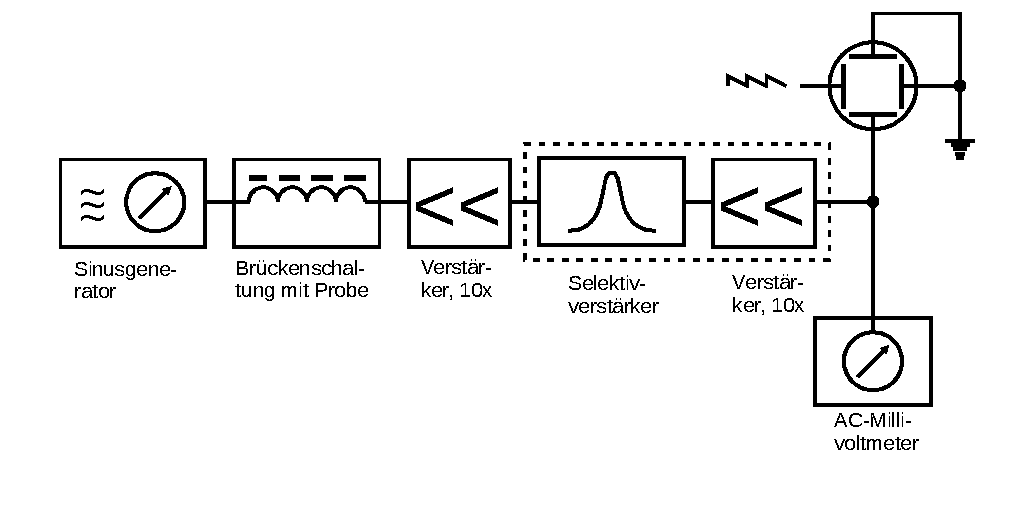
\includegraphics{figures/Abb_5.pdf}
    \caption{Blockschaltung der Messaperatur}
    \label{fig:abb5}
\end{figure} 

Die Eingangsspannung wird durch einen Frequenzgenerator erzeugt.
Die Verstärker vor und hinter dem Selektivverstärker aus \autoref{fig:abb5} werden nicht verwendet. 
Die Eingangsspannung wird allerdings am Selektivverstärker 10-fach verstärkt. 
Der Selektivverstärker ist mit einem Spannungsmessgerät verbunden, das über diesen die Brückenspannung $ U_{Br}$ misst.\\

Bei der Messung wird wie folgt vorgaganen: Die Brücke wird ohne Probe abgeglichen, indem das Potentiometer so eingestellt wird, dass die Brückenspannung $U_{Br}$ maximal wird. 
Es werden die Werte des Potenziometers und der Brückenspannung $U_{Br} $ aufgenommen. 
Danach wird die Probe mit dem $\text{Dy}_2\text{O}_3$ in die Spule eingeführt.
Die Brücke wird erneut abgeglichen und die Messwerte für das Potentiometer und die Brückenspannung aufgenommen. Dieses Verfahren wird dreimal wiederholt.\\

Die Messung wird genauso mit $\text{Gd}_2\text{O}_3$ und $\text{Nd}_2\text{O}_3$ wiederholt. Am Ende wird von jeder Probe die Länge gemmessen und das Gewicht abgelesen.\\
